\documentclass[12pt]{article}
\usepackage{amsmath}
\usepackage{amssymb}
%\usepackage[margin=1.2 in, includefoot]{geometry}
\usepackage{color}
\usepackage{rotating}
%\usepackage{setspace}
\usepackage{graphicx}
\author{Zimian Zhang}
\title{Dynamic Models of Cash Management: the 2nd Year's Report}
\begin{document}

%\begin{spacing}{1.0}
\maketitle
\setcounter{page}{0}
\thispagestyle{empty}


\newpage
\tableofcontents
\setcounter{page}{0}
\thispagestyle{empty}

\newpage

\section {Introduction}
\section{A summary of research progress}
\subsection{Introduction}




\subsection{Wrap-up for the 1st year's research}

In cash management research, most literature uses `one asset account' models (e.g. \cite{baccarin2002optimal}, \cite{sato2011stochastic}, \cite{bensoussan2005optimality} and \cite{feng2010computational}). In the `one asset account' setting, companies with only cash account are considered. To be specific, In each time period, managers can adjust the cash holding level with certain transfer fee. Meanwhile, the company will face a certain amount of cash demand. If the current cash holdings cannot meet the cash demand, some shortage cost occurs. On the other hand, a positive cash holdings will also generate some opportunity cost, that is the profits one could get had the manager invested the cash into a profitable asset. The basic idea of `one asset account' models is shown in figure \ref{basic model}.
\begin{figure}
\begin{center}
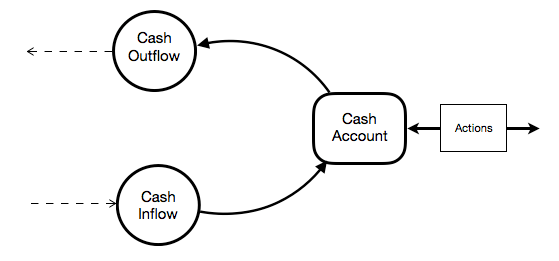
\includegraphics[scale=.6]{basicModel}
\end{center}
\caption{One Asset Account Model}
\label{basic model}
\end{figure}
The limitation of this model is that both cash flows are considered exogenous, i.e. cash outflows or inflows cannot be affected by the policy adopted by managers. 


In light of this, we proposed a two-assets cash management model in our first year's research (see figure \ref{twoAsset}). In this model, managers can transfer any amount of money between cash account and asset account with a fixed amount of transaction fee($\Gamma$). We assumed that at the beginning of each time period, the company will receive some cash as business revenue ($rr \cdot y_t$) whose amount is proportional to the current size of its asset account. Moreover during each time period, a normally distributed stochastic amount of cash demand occurs($D$). If the cash demand exceeds current cash holdings, managers have to sell their asset to offset the cash deficit along with a fixed amount of cash shortage penalty($SC$). The objective function of this model is to maximise the total cash inflow for the infinite time horizon. 

The advantage of this model is that the size of cash inflow are affected by managers actions. Moreover, compared with one asset account models, the profit of investing money into asset rather than holding as cash is calculated compounded in this model. Figure \ref{firstY} shows one result of this model.






\begin{figure}
\begin{center}
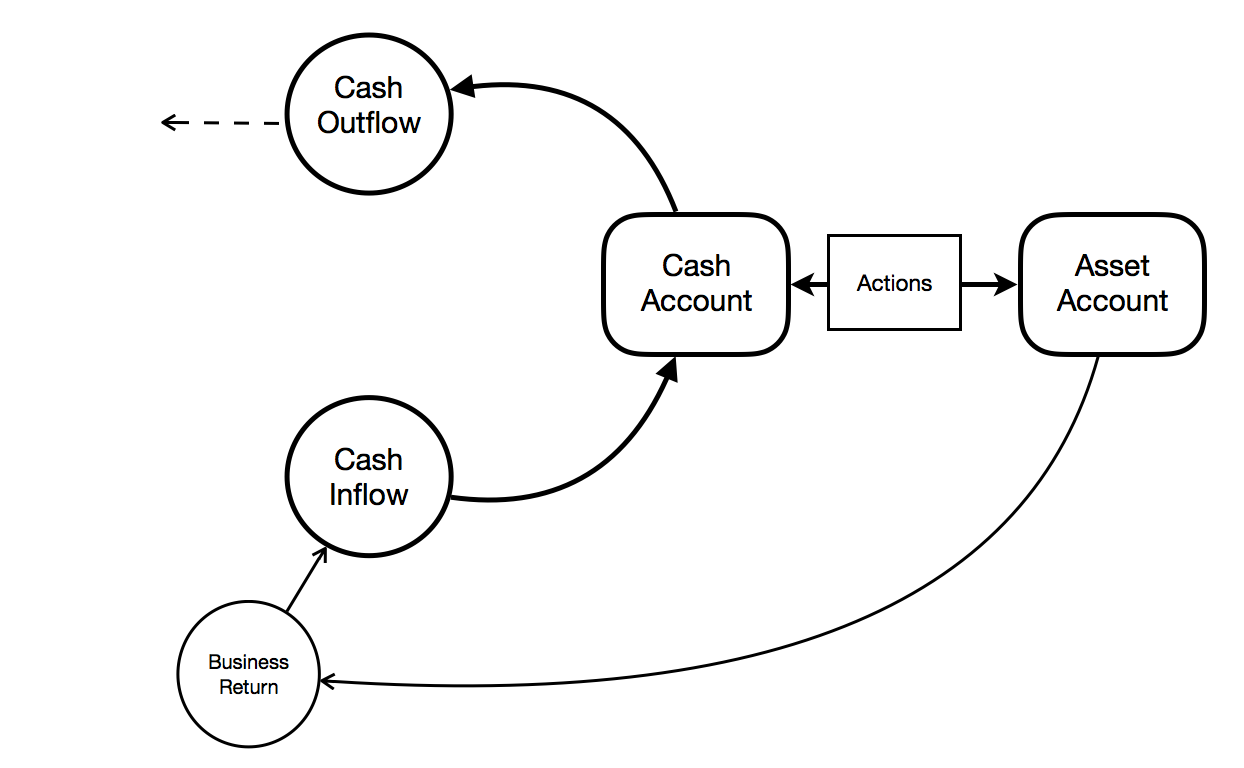
\includegraphics[scale=.5]{twoAssets}
\end{center}
\caption{Two Asset Accounts Model}
\label{twoAsset}
\end{figure}


\begin{figure}
\begin{center}
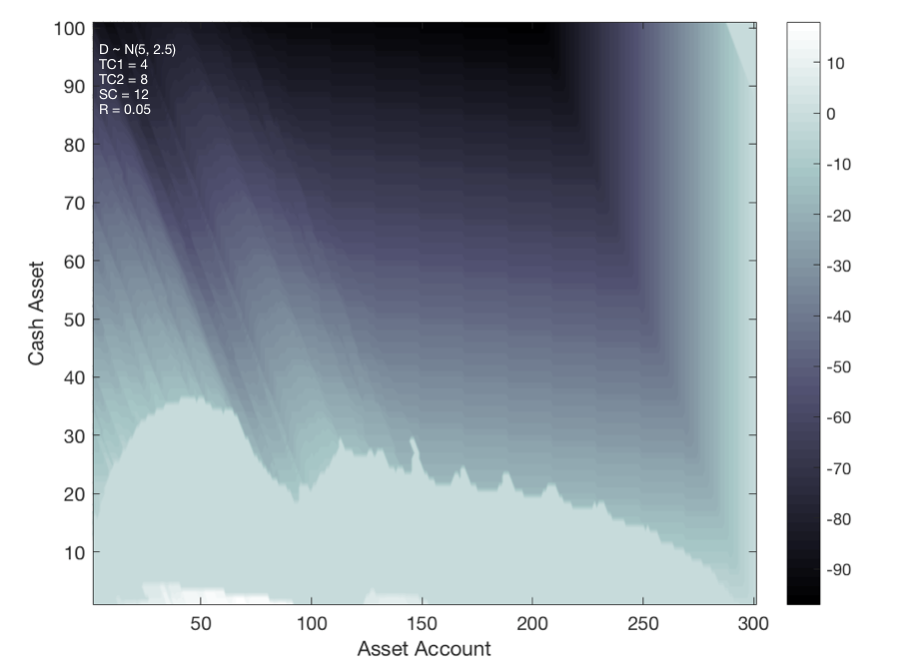
\includegraphics[scale=.3]{ResultFirstYear_rdy}
\end{center}
\caption{A Optimal Solution of the Two Accounts Model}
\label{firstY}
\end{figure}

\subsection{Model modification}
In order to fit the real world better, we made several modifications. To begin with, we changed the objective function from maximising total revenue to maximising net profits: $$\max \sum^T_{t = 0}\gamma^t  \{ rr \cdot y_t - D_t - \Gamma_t - SC_t \}.$$ We made this change since net profit can describe the performance and profitability of a company better and thus maximising the net profit are normally managers main goal. The second modification is that we adopted a transfer cost function that is partially fixed and partially proportional to the amount of transaction. This new function can be expressed by the following formula: $$\Gamma(a) =  (K_c + k_c a) \cdot 1_{\{ a < 0\}} + (K_a +k_aa)\cdot 1_{\{a>0\}}$$ where $a$ is the amount of money transferred from asset account to cash account (negative value means the other way around); $K_c$ and $K_a$ are the fixed part of the transaction cost function while $k_c$ and $k_a$ are the parameters in the proportional part. The rationale of this modification can be explained as this: In the need of cash, the manager might want to sell some illiquid asset. This action would require two different costs: a fixed cost regardless of the amount of asset he want to sell, e.g. advertising expense, salesmen's salaries etc. and a proportional cost since illiquid assets are normally sold at lower price than its true value. Similar costs apply to the disposal of cash to get profitable assets. In financial sector, brokerage commission, which is one of the main sources of transaction cost, are also normally partially fixed and partially proportional to the transaction amount.

Moreover, we added transaction cost into shortage cost. When a company face a amount of cash demand which exceeding its current cash level, the manager has to sell enough assets to offset the cash deficit and to pay the shortage cost: $$SC = (SP + \Gamma(D-x')) \cdot 1_{\{D>x'\}}.$$ The shortage cost consists of two parts: a fixed amount of shortage penalty and the transaction cost generated by selling asset to offset cash deficit. 

At last, we allow managers to declare bankruptcy at any point of time. Once the manager declared bankruptcy, the net profit in that time period as well as the amount of both accounts will be set as zero. Figure \ref{ModifiedModel} shows one result of our modified model.

\textcolor{red}{Add analysis here...}


\begin{figure}
\begin{center}
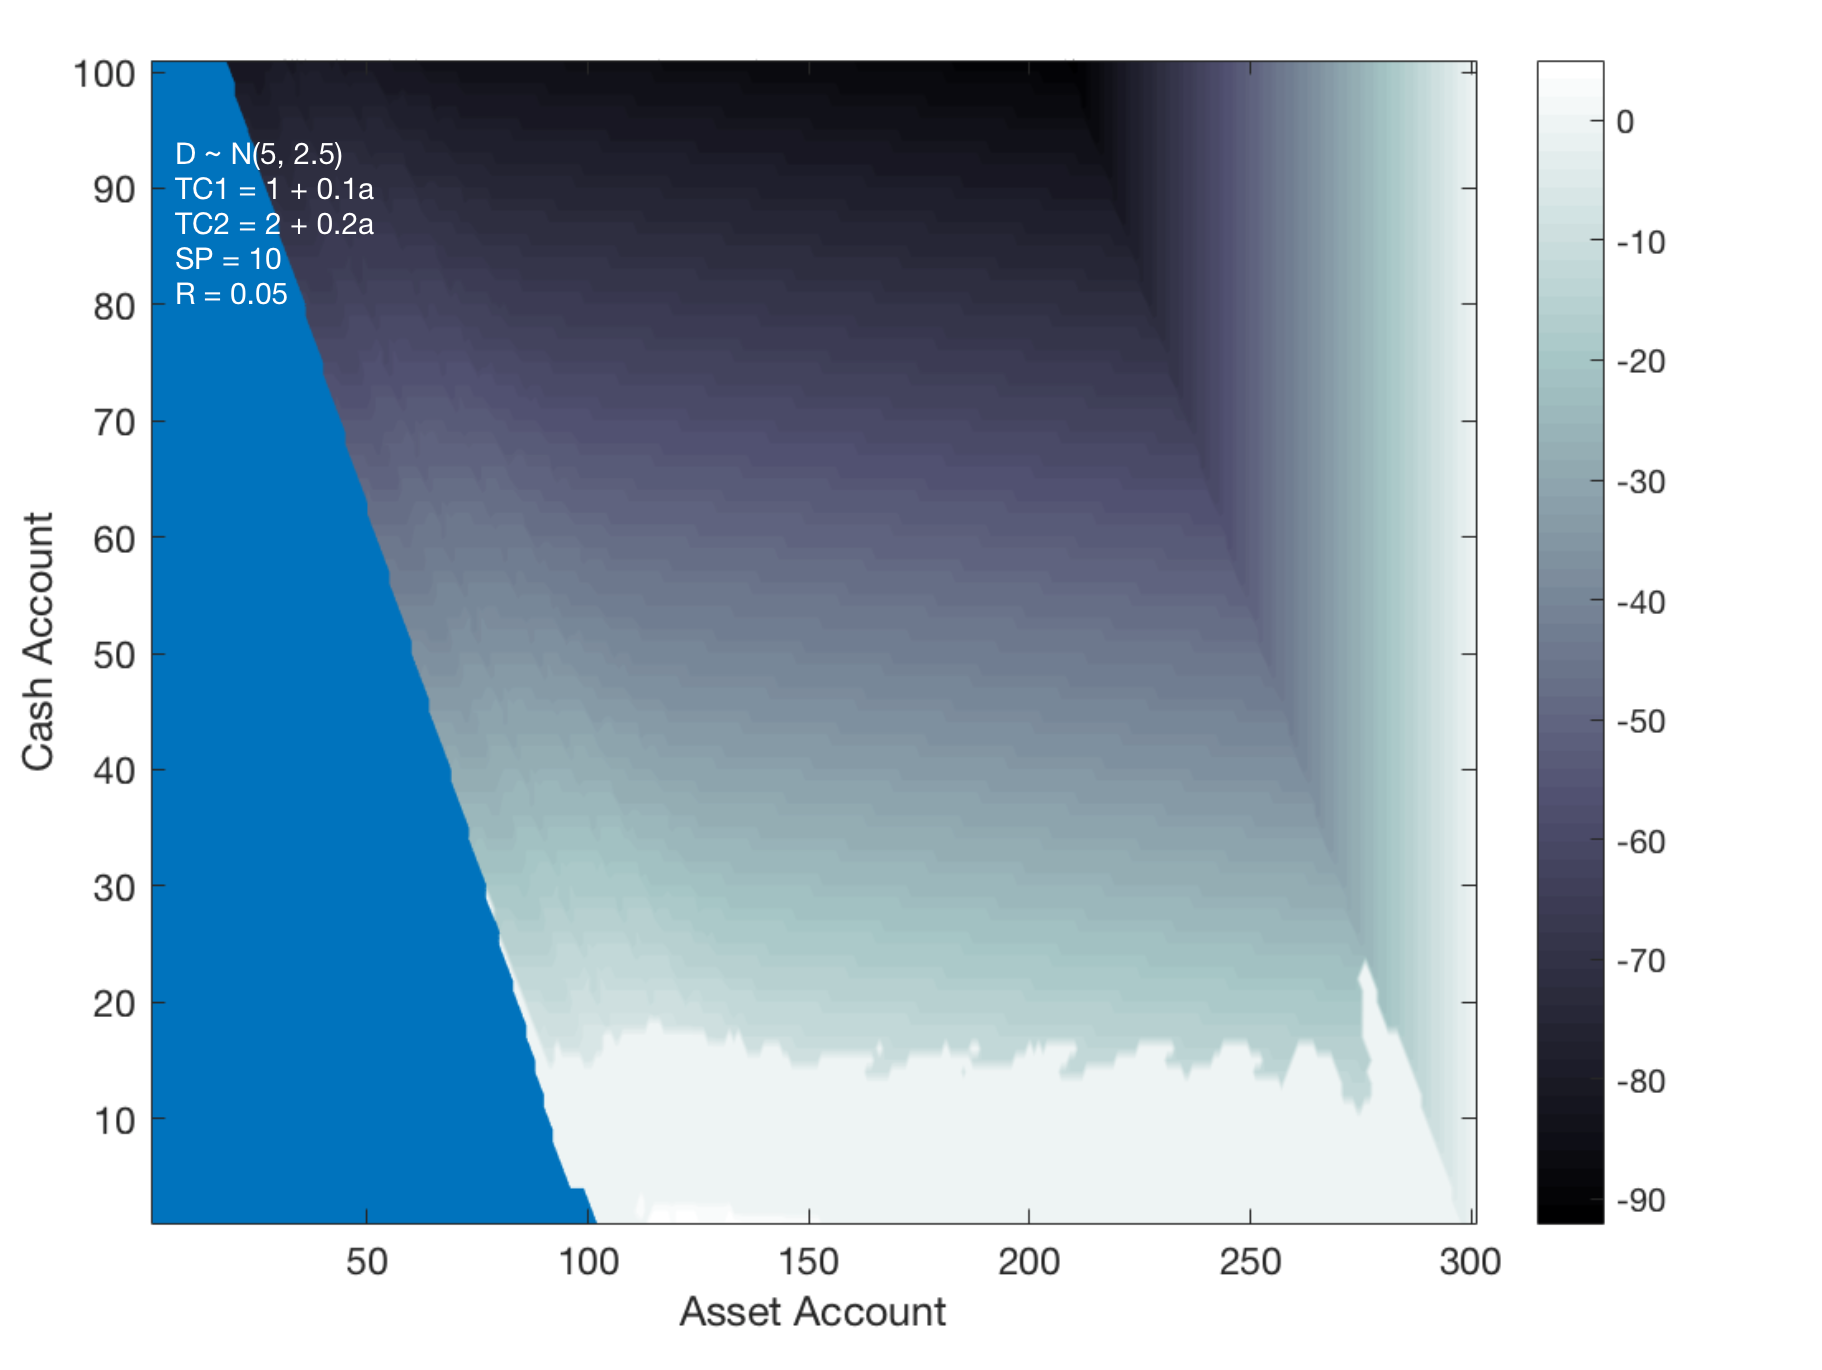
\includegraphics[scale=.3]{ModifiedModel}
\end{center}
\caption{A Optimal Solution of the Modified Model}
\label{ModifiedModel}
\end{figure}



\subsection{Model evaluation: simulation and bankruptcy probabilities}
We run several simulations to evaluate the policies generated by our model. Figure \ref{simulation} shows the results of 100 simulations in four different experiments. Each experiments has the same model parameters: Cash demand is normally distributed with $\mu=5.0$, $\sigma=2.5$; business return rate is $0.05$; shortage penalty is $10$ and transaction cost function has parameters$K_c = 1.0$, $k_c=0.1$,$K_a=2.0$ and $k_a=0.2$; In each simulation experiment, the manager follows the policy suggested by the dynamic programming model. The starting states for these experiments are $S = (10,90)$,$S=(10,100)$, $S=(10,110)$ and $S=(10,120)$ respectively. It can be seen that while the initial states are relatively close to each other, the results are significantly different. This suggested that in our model, given that the optimal policy is adopted, companies are highly likely go to bankruptcy once they are in a `slightly bad position' (such as state 10,90) and once they are in a 'slightly good position' (such as state 10, 120) things are very unlikely to go bad.

\begin{figure}
\begin{center}
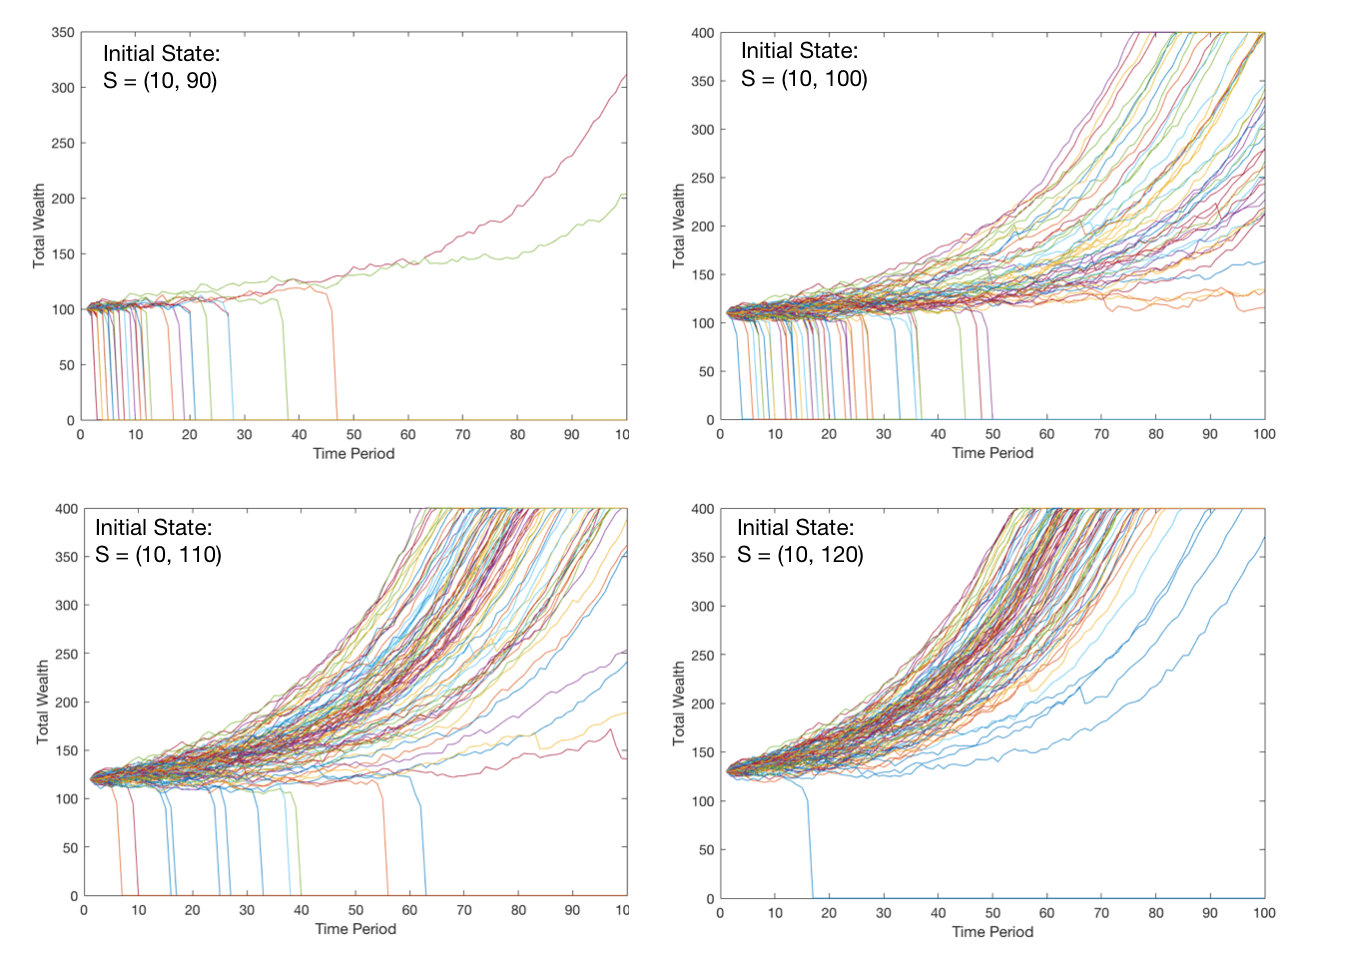
\includegraphics[scale=.56]{simu}
\end{center}
\caption{Simulation Results at Different Initial State}
\label{simulation}
\end{figure}

To examine the performance of this cash management policy more holistically, we propose a backward method to calculate the bankruptcy probability in our model. At the end the time horizon (stage 0), if the company has a non-negative cash account or has enough asset to offset its deficit, one can claim that this company does not go to bankruptcy (i.e. with probability 0 to go to bankruptcy). In other words, at stage 0, any state $S_{[x, y]}$ with $y \neq 0$ has value (probability of bankruptcy) equal to 0 and any state $S_{[x, y]}$ with $y = 0$ has value (probability of bankruptcy) equal to 1. 

At stage 1, the value of state $S_{[x, y]}$ equals the probability of going bankruptcy in this time period plus the probability of going bankruptcy in next time period (i.e. the sum of the product of the probability that the company go to stage $S_{[x', y']}$ next time period (stage 0) and the value (probability of bankruptcy) in that state at stage 0 for all possible $x'$ and $y'$. )

Therefore at stage 1, the probability of eventually going bankruptcy for each state can be written as: 

\[
\begin{split}
V_{[x,y]}^{t=1} =& \sum P\left\{\left.S_{(0,0)}:W(S_{x,y}) = S_{(0,0)}\right|a = A^*(S_{x,y})\right\} 
\\ 
+ & \sum P\left\{ \left. S_{x',y'}:W(S_{x,y}) = S_{x',y'} \right| a = A^* (S_{x,y})\right\}  V_{[x',y']}^{t=0}
\end{split}
\]

Similarly, the value for any stage $k: k \geq 1$ can be written as

\[
\begin{split}
V_{[x,y]}^{t=k} =& \sum P\left\{\left.S_{(0,0)}:W(S_{x,y}) = S_{(0,0)}\right|a = A^*(S_{x,y})\right\} 
\\ 
+ & \sum P\left\{ \left. S_{x',y'}:W(S_{x,y}) = S_{x',y'} \right| a = A^* (S_{x,y})\right\}  V_{[x',y']}^{t=k-1}
\end{split}
\]
 
 
  Continuing this iteration until the maximum different between two successive stages' values is smaller than a small number $\epsilon =  0.0001$. In the above equations, $P\left\{ \left. S_{x',y'}:W(S_{x,y}) = S_{x',y'} \right| a = A^* (S_{x,y})\right\}$ is the probability that the company goes from state  $S_{x,y}$ to $S_{x',y'}$ when the manager follows the optimal policy $A^*$.
  
Figure \ref{prob} shows the probability of going bankruptcy when a company follows the optimal cash management policy. The right graph is the result calculated by the recursive method proposed above. The left graph is the probability of going bankruptcy generated by 10,000 simulations. It can be seen that the two results are quite similar: both probabilities jump from $1.0$ to $0.0$ very quick. This result suggest that once the optimal cash policy is adopted, most companies will either go to bankruptcy or go to a `safe position' where it is almost impossible for the companies to get worse, depending on which states are they currently in.



\begin{figure}
\begin{center}
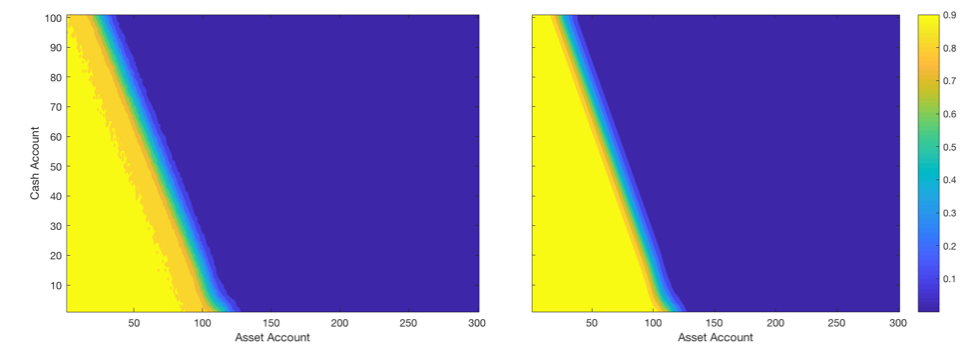
\includegraphics[scale=.40]{prob}
\end{center}
\caption{Probabilities of going bankruptcy in each state}
\label{prob}
\end{figure}




\subsection{Cash management model with loans}
As we discussed in the former section, the optimal cash management policy could help those companies currently in `good position' get to a safe status where it is almost impossible for companies to go to bankruptcy. However, once companies get into a `bad position', the business revenue cannot cover the cash demand. Managers has to sell his asset to meet the current demand, which would deteriorate the companies' profitability further. 

In reality, however, once companies' income could not cover its cash demand, instead of selling asset and jeopardising future profitabilities, managers tend to take loans from other companies or financial intermediaries. In light of this, we propose a two-asset accounts model with loan options. Figure \ref{loan} shows the basic idea of this model. 

\begin{figure}
\begin{center}
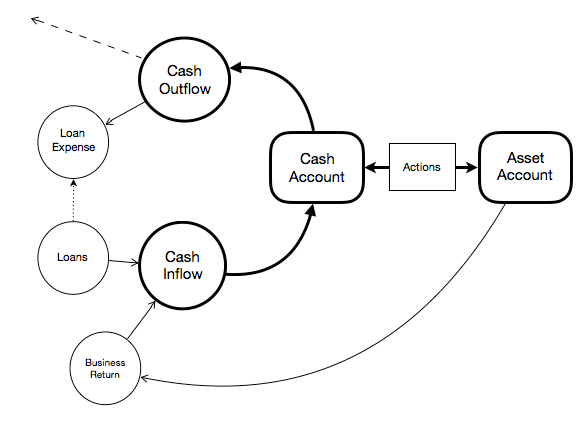
\includegraphics[scale=.43]{loan}
\end{center}
\caption{Two Asset Accounts Model with Loan Options}
\label{loan}
\end{figure}

In addition to the normal two asset accounts model, we add a 'taking loan' option in the model i.e. at any point of time, the manager could take a loan from financial companies. Once a loan was taken, a certain amount of loan repayment must be paid in every following time period until the debt (loan and interest) is offset.   

For simplicity's sake, we assume that there is only one type of loans available in the market and a company is not allowed to take another loan while its debt has not been offset. Let he loan size be $L$ and the interest rate be $lr$. We also assume that once the loan is taken, one must pay a fixed amount $LP$ in each one of the following $N$ time periods. So in each time period, the loan expense can be written as: $$LP = L \cdot \frac{lr \cdot (1+lr)^N}{(1+lr)^N-1}$$
 
 We also formulated this model as a Markov Decision Process where each state consists of three parameters: $S_{x,y,z}$ where $x$ and $y$ represent the current cash and asset level and $z$ represent the remaining times of loan repayment. For example, at time period $t$, a manager takes the loan. Then at time $t+1$ the $z$ value of the company's state changes from $0$ to $N$. In the following periods, the company's cash demand will increase by $LP$ amount and after each period, $z$ value will decrease by $1$ until it gets to $0$. Moreover, the action space also need some modification. Now the action space consists of two parameters: $a_c$ (the amount of money transfer between cash and asset) and $a_l$ (can only take values 0 or 1, indicating whether take the loan or not). Since we assumed that one cannot take loans had his debt not been fully paid, $a_l$ cannot take the value of 1 when $z \neq 0$.
 
 \textcolor{red}{results shown here...}


\subsection{A heuristic method: one-step policy improvement}
One limitation of using Markov Decision Process to solve the cash management model with loan options is the high calculation cost. It took more than 10 hours to get the optimal solution with the assumption of one loan available. To expand the model to a model with multi-loan options, the calculation time will growth exponentially. Thus we propose a heuristic method called one-step policy improvement to get an approximate solution.
\begin{figure}
\begin{center}
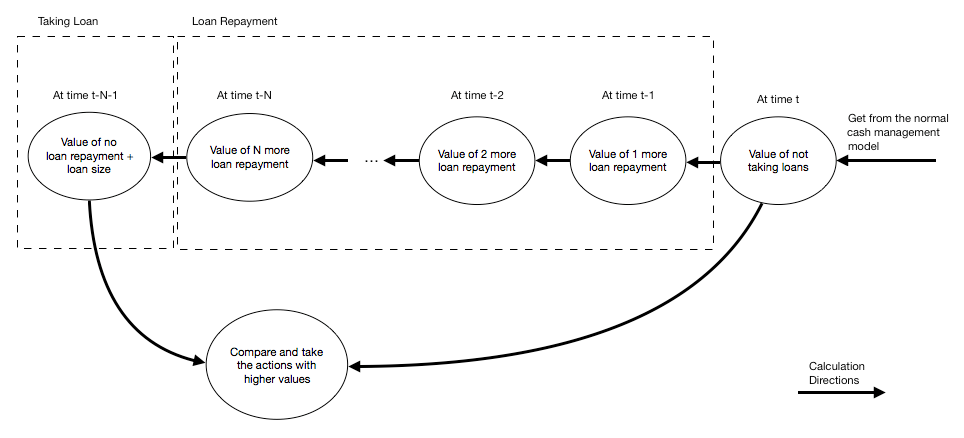
\includegraphics[scale=.4]{oneImprov}
\end{center}
\caption{One Improvement Policy}
\label{oneImprov}
\end{figure}

The basic idea of one-step policy improvement is shown in figure \ref{oneImprov}. The main task is to calculate the value of each cash-asset state conditioning on that the manager has decided to takes loans in the current time period and will never takes loan again. The value of state $S_{x,y}$ given the fact that the manager has decided to take the loan at the current time period and will follow the optimal cash management action $a'_c$ can be denoted by the notation: $$V^{{a_c}', a_l = 1}(S_{x,y}).$$
Then compare this value with the value in the same state but without taking loans in the whole time planning horizon, denoted by the notation: $$V^{{a_c}, a_l = 0}(S_{x,y}).$$ where $a_c$ is the optimal cash management policy without any loan opportunity. So this strategy is the same with the cash strategy from the normal Cash DP model ($a$). Correspondingly, the value $V^{{a_c}, a_l = 0}(S_{x,y})$ is the same with the value from the normal Cash DP model $V^a(S_{x,y}).$


In the normal Cash DP model, we have that $$V^{a_c, a_l =0}(S_{x,y})= V^a(S_{x,y}) =    \gamma R_t^{a}(S_{x,y}) + \gamma \sum_{S_{x',y'}\in S} V^{a}_{t-1}(S_{x',y'})
\mathbb{P}\left\{S_{x',y'}:W(S_{x, y}) = S_{x', y'} \right\}$$

In the above equation, $R^{a}_t(S_{x,y})$ is the return function and can be represent as:$$ R^{a}_t(S_{x,y}) = rr*y - \Gamma(a) - \mathbb{E}[D+SP(S_{x,y},a)]$$


We define $N$ as the total number of loan repayment one has to make. $a_{c, z}$ is the optimal cash management action when there is $z$ loan repayment left,  $L$ is the size of the loan and $lr$ is the corresponding loan interest rate. So we have 

$$V^{a_c', a_l = 1}(S_{x,y}) = L+R^{a}(S_{x+L,y}) + \gamma \sum_{S_{x',y'}\in S }V^{a_{c,z=N}}(S_{x',y'}) \mathbb{P}\left\{ S_{x',y'} : W(S_{x+L,y}=S(x',y')\right\}$$



Let $LP$ be the loan payment in each time period. Now the value of  $V^{a_{c,z=N}}(S_{x+ls, y})$ could be calculated recursively: 
$$a_{c,1} = \arg \max_{a_{c,1} \in \Pi} \gamma [R^{a_{c,1}} (S_{x,y}) - LP] + \gamma  \sum_{S_{x',y'}\in S} V^a(S_{x',y'})\mathbb{P}\left\{S_{x',y'}\widehat{W}(S_{x-LP, y}) = S_{x', y'} \right\}$$
$$ V^{a_{c,1}}(S_{x,y}) = \gamma [R^{a_{c,1}} (S_{x,y}) - LP] + \gamma  \sum_{S_{x',y'}\in S} V^a(S_{x',y'})\mathbb{P}\left\{S_{x',y'}:\widehat{W}(S_{x-LP, y}) = S_{x', y'} \right\}$$

$$a_{c,2} = \arg \max_{a_{c,2} \in \Pi} \gamma  [R^{a_{c,2}} (S_{x,y}) - LP]  + \gamma  \sum_{S_{x',y'}\in S} V^{a_{c,1}}(S_{x',y'}) \mathbb{P}\left\{S_{x',y'}:\widehat{W}(S_{x-LP, y}) = S_{x', y'} \right\}$$
$$ V^{a_{c,2}}(S_{x,y}) = \gamma  [R^{a_{c,2}} (S_{x,y}) - LP]   + \gamma  \sum_{S_{x',y'}\in S} V^{a_{c,1}}(S_{x',y'}) \mathbb{P}\left\{S_{x',y'}:\widehat{W}(S_{x-LP, y}) = S_{x', y'} \right\}$$

$$...$$

$$a_{c,N-1} = \arg \max_{a_{c,N} \in \Pi} \gamma [R^{a_{c,N-1}} (S_{x,y}) - LP] + \gamma  \sum_{S_{x',y'}\in S} V^{a_{c,N-2}}(S_{x',y'}) \mathbb{P}\left\{S_{x',y'}:\widehat{W}(S_{x-LP, y}) = S_{x', y'} \right\}$$
$$ V^{a_{c,N-1}}(S_{x,y}) = \gamma [R^{a_{c,N-1}} (S_{x,y}) - LP] + \gamma  \sum_{S_{x',y'}\in S} V^{a_{c,N-2}}(S_{x',y'}) \mathbb{P}\left\{S_{x',y'}:\widehat{W}(S_{x-LP, y}) = S_{x', y'} \right\}$$

$$a_{c,N} = \arg \max_{a_{c,N} \in \Pi} \gamma [R^{a_{c,N}} (S_{x,y}) - LP] + \gamma  \sum_{S_{x',y'}\in S} V^{a_{c,N-1}}(S_{x',y'}) \mathbb{P}\left\{S_{x',y'}:\widehat{W}(S_{x-LP, y}) = S_{x', y'} \right\}$$
$$ V^{a_{c,N}}(S_{x,y}) = \gamma [R^{a_{c,N}} (S_{x,y}) - LP] + \gamma  \sum_{S_{x',y'}\in S} V^{a_{c,N-1}}(S_{x',y'}) \mathbb{P}\left\{S_{x',y'}:\widehat{W}(S_{x-LP, y}) = S_{x', y'} \right\}.$$

Then for each state, we compare the value of `taking loan once and never take it again' i.e. $V^{a'_c,a_l = 1}(S_{x,y})$ with the value of `not taking loan in the entire planning time horizon' i.e. $V^a(S_{x,y})$. For any state $S_{x,y,z=0}$, if the policy `taking loan once and never take it again' is better than `not taking loan at all', then whenever the system comes to the state $S_{x,y,z=0}$, the loan should be taken.

Then we examine the performance of the one step improvement algorithm using simulation method. Based on the old model settings, we assume that the manager could take a loan with size 40, loan interest rate 0.03. Once the loan is taken, it should be paid within 40 time periods with equal amount of repayment in each time. Figure \ref{OSI} shows the total number of identical companies that did not declare bankruptcy in each time period during total 10,000 simulations. It can be seen that the probabilities for a company not going bankruptcy can be increased when the loan is available on the financial market. Moreover, the performance of the policy suggested by the one-step policy improvement algorithm is quite close to the policy suggested by the dynamic programming method. With respect to calculation time, dynamic programming would take more than 10 hours while the one-step improvement algorithm only take 8 minutes on the same PC. 

Furthermore, with one-step improvement algorithm, one could easily expand the cash management model with single loan option to a model with multi-loan options. Assume there are two possible loan options, i.e. $a_l$ could take value of $0$, $1$ and $2$. Let $a_l = 0$ represent the manager does not take any loans, $a_l=1$ represent that he take the first loan and do not take any loan thereafter, $a_l=2$ represent that he take the second loan and do not take any loan thereafter. By using one-step policy improvement, one need to calculate $V^{a'_c, a_l=1}(S_{x,y})$ and $V^{a'_c, a_l=2}(S_{x,y})$ separately for each state $S_{x,y}$. Then for each state, the highest value among $V^a(S_{x,y})$, $V^{a'_c, a_l=1}(S_{x,y})$ and $V^{a'_c, a_l=2}(S_{x,y})$ should be recorded along with its corresponding actions. The recorded policy is the policy suggested by one-step policy improvement algorithm. 


\begin{figure}
\begin{center}
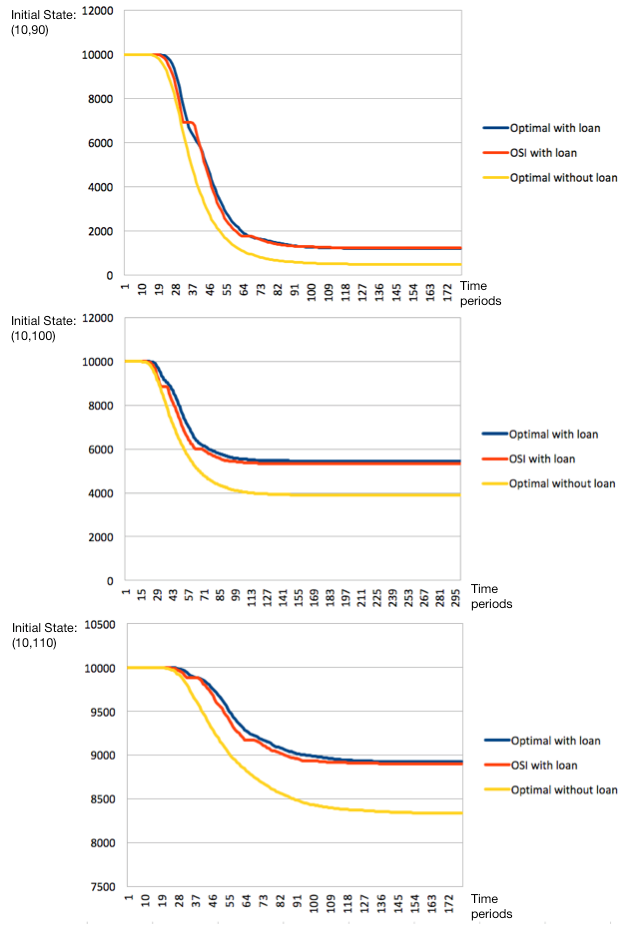
\includegraphics[scale=.6]{OSI}
\end{center}
\caption{Survival Companies with Different Policies}
\label{OSI}
\end{figure}












\subsection{Holistic model}
So far we discussed two sources of cash inflows (i.e. business revenue and loans) and one sources of cash demand (i.e. loan expense) in our cash management model. We assumed there is no other sources of cash inflows and assumed the other cash demand is exogenous. But in the real world, cash flows in a company could be much more complicated. Thus we propose a holistic model to discuss the cash flows and management strategies with more details.

The basic idea of the holistic model is shown in figure \ref{Holistic}. To begin with, we consider capital asset and liquid asset separately. Liquid asset (such as raw material for manufacturers and portfolio for financial companies) are those asset that can be relatively easily sold for cash. The amount of liquid asset holdings can affect business income directly. Capital asset, on the other hand, are those assets that cannot be easily sold with a good price and do not affect companies profitability in short terms (e.g. manufacture equipment, branches and employees). However, the capacities of holding liquid asset depends on the size of capital asset account. For example, one manufacture equipment can only process a certain amount of raw material; one broker can only serve a number of customers. Should managers want to increase the capacity of liquid asset (process more raw materials or attract more customers), the size of capital asset must be increased. Meanwhile the capital asset generate another source of cash demand: operation expense. For example, more manufacture equipments require higher maintenance fees; a new branch office would cause higher utility bills; a company usually spend a lot of money to hire and train a new employee. 

In addition to business revenue and taking loans, we would like to introduce another sources of cash inflows: taking financial investment. In a well developed financial market, 



\begin{figure}
\begin{center}
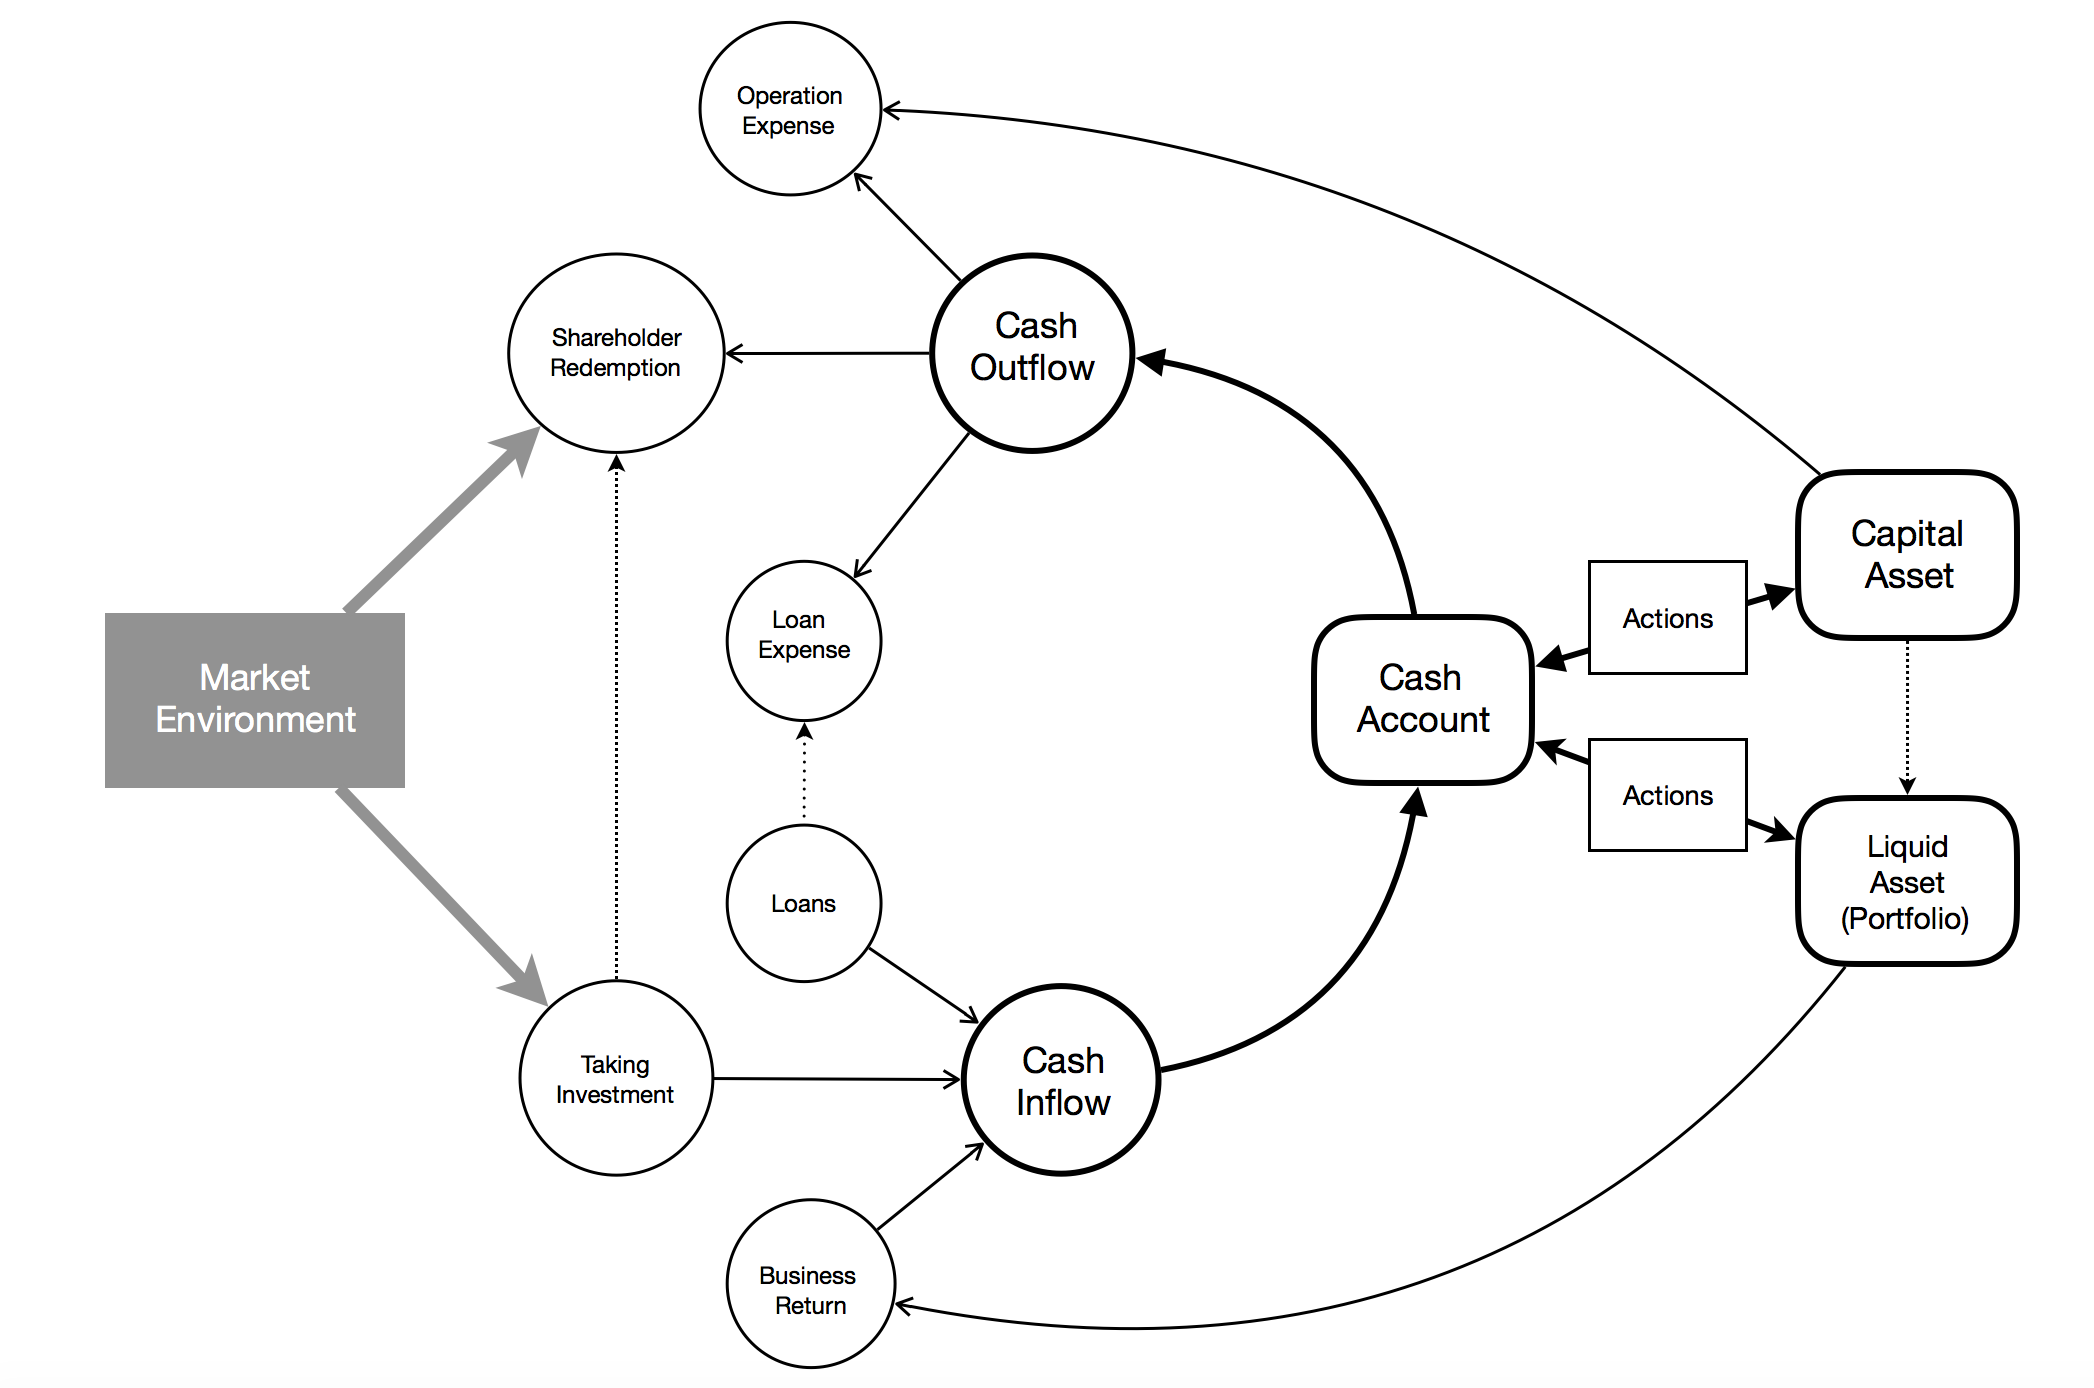
\includegraphics[scale=.33]{Holistic}
\end{center}
\caption{Cash Flows in a Holistic Model}
\label{Holistic}
\end{figure}


\subsection{Approximate dynamic programming: TD method and eligibility trace method}






\section{Overall research project}
\subsection{Introduction}
\subsection{Outline of the thesis}
\subsection{Novelty and possible contributions}
\section{Risk management}
\section{Attendance of PhD level training courses and other related actions}








\section{Time table for third year}




\newpage
\bibliographystyle{plain}
\bibliography{BibliographyinCashProblem}
%\end{spacing}
\end{document}